\documentclass[12pt,notes=off,unicode]{beamer}
\usepackage[italian]{babel}
\usepackage[utf8]{inputenc}
\usepackage{xcolor}
\usepackage{fancyhdr}
\usepackage{amsthm}
\usepackage{amsmath}
\usepackage{amssymb}
\usepackage{mathtools}
\usepackage{lmodern}
\usepackage{tikz}
\usepackage{siunitx}
\usepackage{eurosym}
\usepackage{braket}
\usepackage{animate}

\usepackage{listings}
\usepackage{color}
\definecolor{mygreen}{rgb}{0,0.6,0}
\definecolor{mygray}{rgb}{0.5,0.5,0.5}
\definecolor{mymauve}{rgb}
{0.58,0,0.82}

\lstset{ %
  backgroundcolor=\color{white},   % choose the background color
  basicstyle=\tiny\ttfamily,        % size of fonts used for the code
  language = Python,
  breaklines=true,                 % automatic line breaking only at whitespace
  captionpos=b,                    % sets the caption-position to bottom
  escapeinside={\%*}{*)},          % if you want to add LaTeX within your code
  stringstyle=\color{mymauve},     % string literal style
  keywordstyle=\color{blue},       % keyword style
  otherkeywords={True},
  identifierstyle=\color{red},
  %deleteidentifiers={StopIteration},
  commentstyle=\color{mygray},    % comment style
}

\usetikzlibrary{decorations}
\usetikzlibrary{er}

\graphicspath{{./img/}}

\usetheme{Frankfurt}
\setbeamercovered{dynamic}

\title{Internship report}
\author[Ruggero]{Ruggero Lot}
%\date[]{}

\institute[SISSA]{International School for Advanced Studies}
\logo{
\includegraphics[scale=0.02]{sissa_logo}}



\setbeamertemplate{headline}
{%
  \leavevmode%
  \begin{beamercolorbox}[wd=.5\paperwidth,ht=2.5ex,dp=1.125ex]{section in head/foot}%
    \hbox to .5\paperwidth{\hfil\insertsectionhead\hfil}
  \end{beamercolorbox}%
  \begin{beamercolorbox}[wd=.5\paperwidth,ht=2.5ex,dp=1.125ex]{section in head/foot}%
    \hbox to .5\paperwidth{\hfil\insertframenumber/\inserttotalframenumber\hfil}
  \end{beamercolorbox}%
}


\setbeamertemplate{footline}
{
  \leavevmode%
  \hbox{%
  \begin{beamercolorbox}[wd=.333333\paperwidth,ht=2.25ex,dp=1ex,center]{section in head/foot}%
    \usebeamerfont{title like}\insertinstitute
  \end{beamercolorbox}%
  \begin{beamercolorbox}[wd=.333333\paperwidth,ht=2.25ex,dp=1ex,center]{section in head/foot}%
    \usebeamerfont{title in head/foot}\insertsubsection
  \end{beamercolorbox}%
  \begin{beamercolorbox}[wd=.333333\paperwidth,ht=2.25ex,dp=1ex,right]{section in head/foot}%
    \usebeamerfont{date in head/foot}\insertauthor \hspace*{2ex} 
  \end{beamercolorbox}}%
  \vskip0pt%
}

\setbeamertemplate{navigation symbols}{}

\begin{document}

  \begin{frame}[noframenumbering, plain, c]\frametitle{}
    \maketitle
    \small
    \begin{tabular}{l l}
      tutor: & Prof. Stefano de Gironcoli\\
      tutor: & Ph.D. Emine K\"{u}\c{c}\"{u}kbenli\\
      university tutor: & Prof. Maria Peressi
    \end{tabular}
  \end{frame}

  \section{the big picture} % (fold)
  \label{sec:the_big_picture}

  \begin{frame}[c]\frametitle{CSP}
      
    \begin{center}
      Ab initio - Crystal structure prediction
    \end{center}
    \only<2->{
    \textbf{Key challenge}
    \begin{itemize}
      \item computational cost of thermodynamical exploration
      \item accuracy needed to solve similarly-low energies among polymorphism 
    \end{itemize}
    }
    \only<3->{
    We will focus mostly on the first one exploring  new techniques to reduce the computational cost.
    }
  
  \end{frame}

  \note{the field we are working on is the CSP one in the particular case of Ab initio csp. So what is CSP, as the name suggest: given a molecule or a set of atoms find how they will crystallize. Why ab initio? well because all the calculation are carried out without experimental parameters.}

  \begin{frame}[c]\frametitle{Our tools for CSP}
      
    \begin{center}
      \textbf{USPEX}
      $\iff$
      \textbf{QUANTUM ESPRESSO}
    \end{center}
    \begin{columns}
      \column{.5\textwidth}
      USPEX\\
      (Universal Structure Predictor: Evolutionary Xtallography)\\
      for crystal structure proposal\\
      \column{.5\textwidth}
      QE\\
      for physics\\
    \end{columns}
  \end{frame}
  
  % section the_big_picture (end)

  \section{tools overview} % (fold)
  \label{sec:tools_overview}
    \begin{frame}[c]\frametitle{USPEX}
        
      \begin{columns}
        \column{.5\textwidth}
        \resizebox{\textwidth}{\textwidth}{%
          \begin{tikzpicture}
            \node (img) {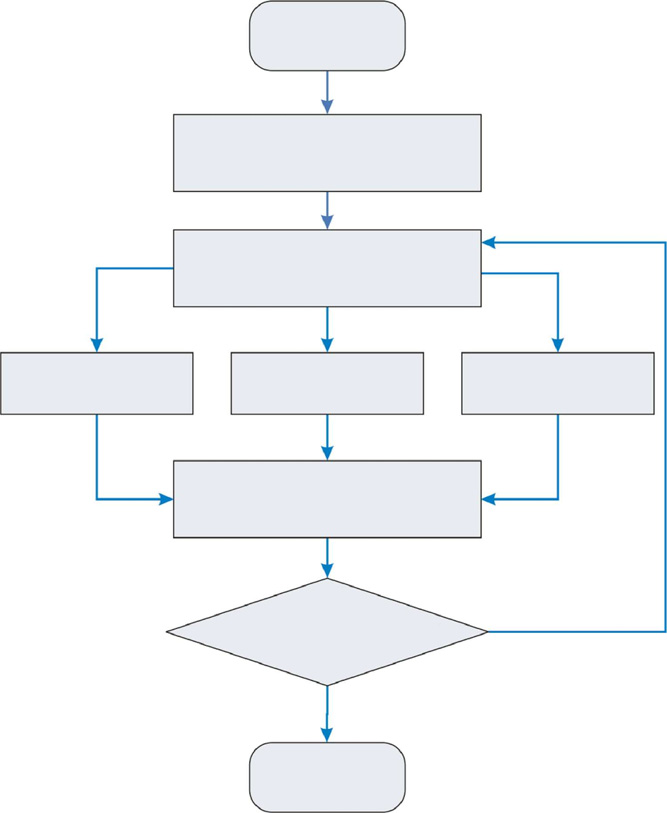
\includegraphics[width=\textwidth]{evo}};
            \node [text width=3cm,align=center] at (-.06,3){\tiny{start}};
            \node [text width=3cm,align=center] at (-.06,2.1){\tiny{Initialisation,}};
            \node [text width=3cm,align=center] at (-.06,1.95){\tiny{first population}};
            \node [text width=3cm,align=center] at (-.06,1.2){\tiny{Create new population}};
            \node [text width=3cm,align=center] at (-1.93,0.2){\tiny{Best individuals}};
            \node [text width=3cm,align=center] at (-.06,0.2){\tiny{Mutation}};
            \node [text width=3cm,align=center] at (+1.88,0.2){\tiny{Heredity}};
            \node [text width=3cm,align=center] at (-.06,-.75){\tiny{New population}};
            \node [text width=3cm,align=center] at (-.06,-1.75){\tiny{Halting criteria}};
            \node [text width=3cm,align=center] at (-.06,-1.9){\tiny{achieved?}};
            \node [text width=3cm,align=center] at (-.06,-3){\tiny{stop}};
          \end{tikzpicture}
        }
        \column{.5\textwidth}
        \textbf{Fingerprint}
        \begin{equation*}
          F_{AB}= \sum_{A_i,cell}\sum_{B_j} \frac{\delta(R-R_{ij})}{4\pi R^2_{ij} \frac{N_A N_B}{V} \Delta} -1
        \end{equation*}
        \textbf{Distance}
        \begin{equation*}
          D_{cos}=\frac{1}{2}\left(1- \frac{\mathbf{F}_1 \cdot \mathbf{F}_2}{|\mathbf{F}_1||\mathbf{F}_2|}\right)
        \end{equation*}
        \begin{tiny}
          
        \end{tiny}
      \end{columns}
      \par\hfill \tiny A. R. Oganov and M. Valle, J. Chem. Phys. 130, 104504 (2009)
    \end{frame}

    \begin{frame}[c]\frametitle{Q.E.}

      \begin{tikzpicture}
        \only<1->{
          \node (img1) {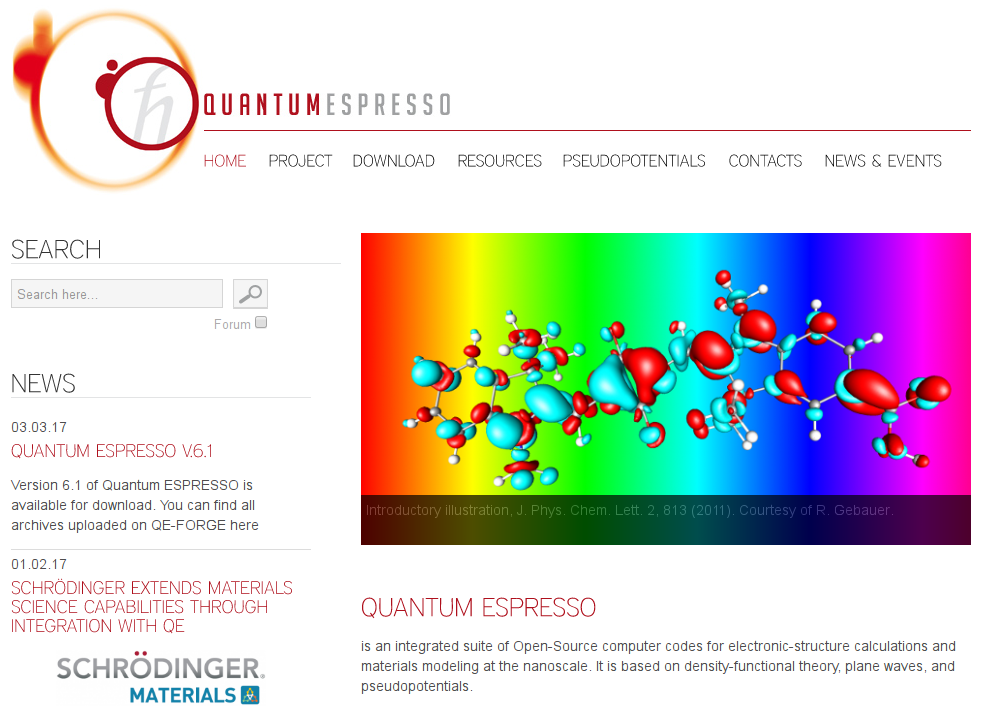
\includegraphics[width=\textwidth]{q1}};
        }
        \only<2->{
          \node (img2) at (2.5,-1) {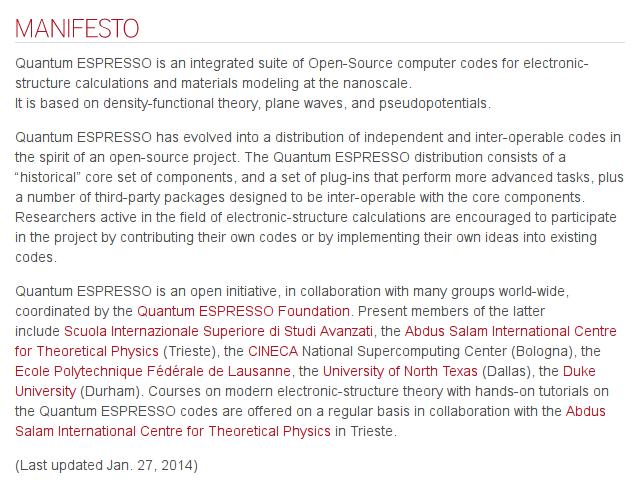
\includegraphics[width=.6\textwidth]{q2}};
        }
      \end{tikzpicture}
        
    \end{frame}

    \begin{frame}[c]\frametitle{HK theorems}
        
      \begin{theorem}
        For any system of interacting particles in an external potential $V_{ext}(r)$, the potential $V_{ext}(r)$ is determined uniquely, except for a constant, by the ground state particle density $n_0(r)$.
      \end{theorem} 
      \begin{theorem}
        A universal functional for the energy $E[n]$ in terms of the density $n(r)$ can be defined, valid for any external potential $V_{ext}(r)$. For any particular $V_{ext}(r)$, the exact ground state energy of the system is the global minimum value of this functional, and the density $n(r)$ that minimizes the functional is the exact ground state density $n_0(r)$.
      \end{theorem} 
    
    \end{frame}
    \begin{frame}[c]\frametitle{KS scheme}
        
      \begin{equation*}
        \begin{matrix}
          \only<1>{
          V_{ext}(r) & \xLeftarrow{HK} & n_0(r) \\
          \Downarrow & ~ & \Uparrow \\
          \{\psi_i(\{\mathbf{r}\})\} & \Rightarrow &\psi_0(\mathbf{\{r\}})\\
          }
          \only<2->{
          V_{ext}(r) & \xLeftarrow{HK} & n_0(r) & \xleftrightarrow{KS} & n_0(\mathbf{r}) & \xRightarrow{HK_0} & V^{KS}(\mathbf{r}) \\
          \Downarrow & ~ & \Uparrow  & ~ & \Uparrow & ~ & \Downarrow\\
          \{\psi_i(\{\mathbf{r}\})\} & \Rightarrow &\psi_0(\{\mathbf{r}\}) & ~ & \psi_{i = 1\dots N_e}(\mathbf{r}) & \Leftarrow & \{\psi_i(\mathbf{r})\} \\
          }
        \end{matrix}
      \end{equation*}
      \only<2->{
      \begin{equation*}
        E^{KS}[n] = T_s[n]+\int d \mathbf{r} V_{ext}(r) n(r) + E^{H}[n] + E^{xc}[n] + E^{II}
      \end{equation*}
      }
      \only<3->{
      \begin{equation*}
        \frac{\delta E[n]}{\delta \psi^\star_l(\mathbf{r})}= \left[-\frac{\hbar^2}{2 m} \mathbf{\nabla}^2 + \overbrace{V^{ext}(\mathbf{r}) + V^{H}(\mathbf{r}) +  v^{xc}(\mathbf{r})}^{V^{KS}(\mathbf{r})}\right] \psi_l(\mathbf{r})
      \end{equation*}
      }
      \only<4->{
      \begin{equation*}
        H^{KS}\ket{\psi_i^{ks}}=e_i \ket{\psi_i^{ks}}
      \end{equation*}
      \par\hfill \tiny we used a vdW-functional
      }
    \end{frame}

    \begin{frame}[c]\frametitle{Self consistency and BFGS}
        
      \begin{columns}
        \column{.5\textwidth}
        \begin{center}
          \resizebox{.6\textwidth}{.6\textwidth}{%
          \begin{tikzpicture}
            \def \radius {3cm}
            \def \margin {17} 

            \node[draw, circle] at (0:\radius) {$V^{KS}(\mathbf{r})$};
            \draw[<-, >=latex] ({0 + \margin}:\radius) 
              arc ({0 + \margin}:{120-\margin +5}:\radius);
            \node[draw, circle] at (120:\radius) {$n(\mathbf{r})$};
            \draw[<-, >=latex] ({120 + \margin -5}:\radius) 
              arc ({120 + \margin}:{240-\margin}:\radius);
            \node[draw, circle] at (240:\radius) {$\{\psi_i(\mathbf{r})\}$};
            \draw[<-, >=latex] ({240 + \margin}:\radius) 
              arc ({240 + \margin}:{360-\margin}:\radius);
          \end{tikzpicture}
          }
        \end{center}
        \begin{align*}
          E_{el} &= -\frac{\hbar^2}{2m}\sum_i \bra{\psi_i}\nabla^2\ket{\psi_i} + E_{ext,H,xc}\left[n\right]\\
          F_{el}^{I\alpha} &= - \frac{\partial E_{el}}{\partial R_{I\alpha}}
        \end{align*}
        \column{.5\textwidth}
        \animategraphics[loop,controls,width=\linewidth]{12}{gif/gif-}{0}{99}
        \begin{tiny}
          BSGF animation, 3 mol/cell, 10Gpa, cell can change. 
        \end{tiny}
      \end{columns}
    \end{frame}
  % section tools_overview (end)

  \section{Already known results} % (fold)
  \label{sec:already_known_results}

    \begin{frame}[c]\frametitle{Results based on these two ideas}
        
      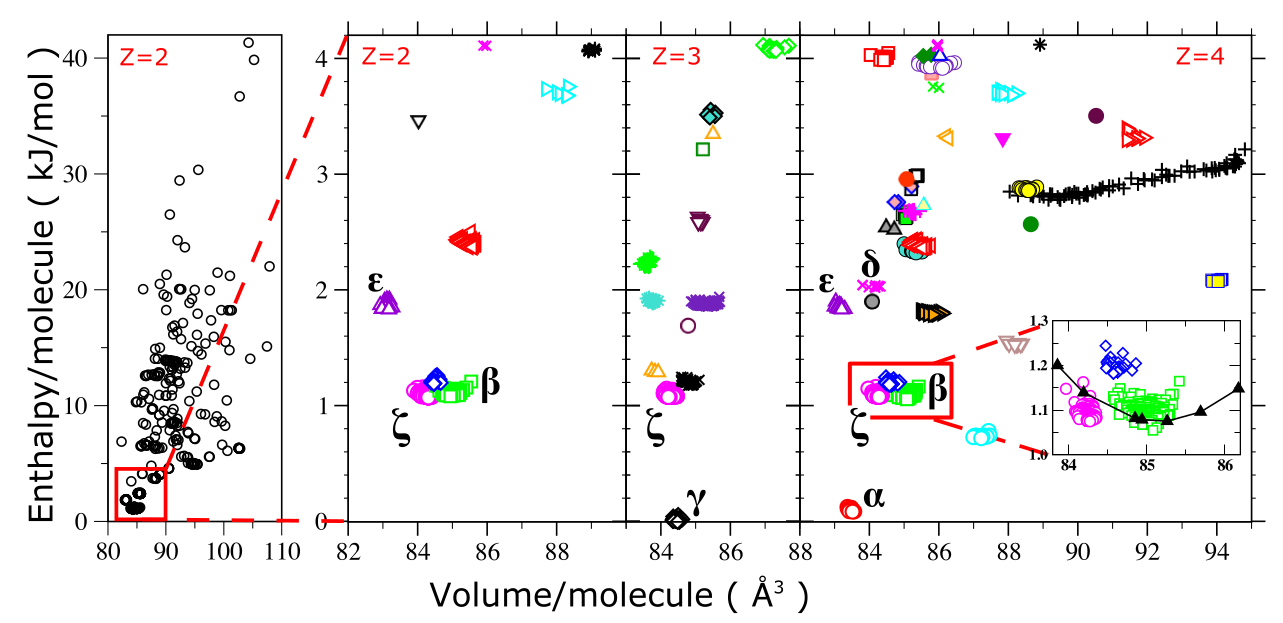
\includegraphics[width=\textwidth]{emine_paper}
      \par\hfill \tiny arXiv:1605.00733 [cond-mat.mtrl-sci]

    \end{frame}

  % section already_known_results (end)

  \section{what we are developing} % (fold)
  \label{sec:what_we_are_developing}
    \begin{frame}[c]\frametitle{Neural network}
        
      \begin{columns}
        \column{.5\textwidth}
        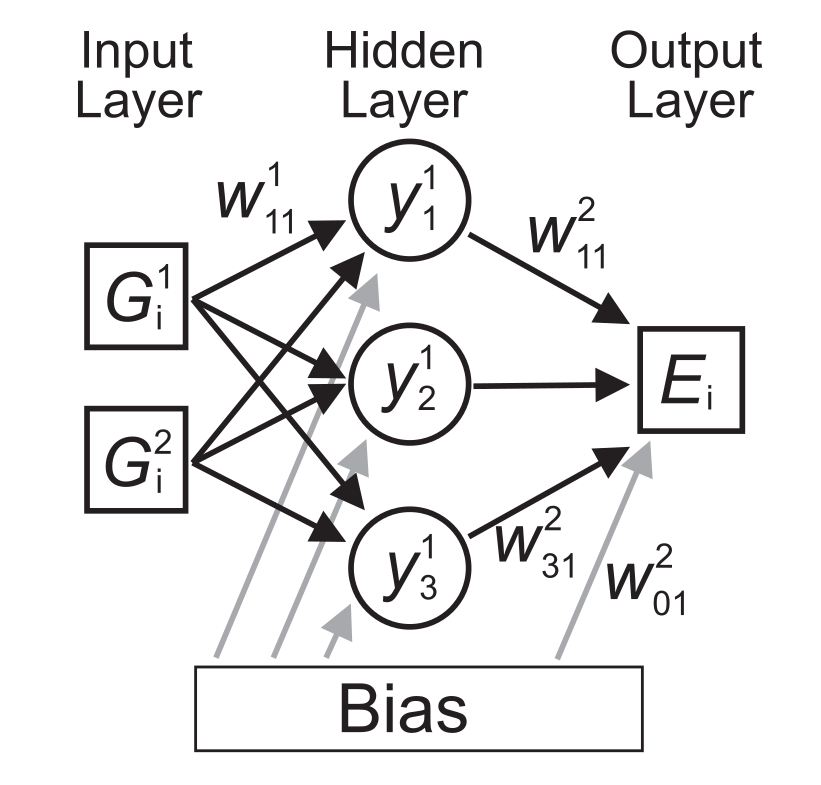
\includegraphics[width=\textwidth]{nn_parinello}
        \column{.5\textwidth}
        Realized function
        \begin{tiny}
          \begin{equation*}
            E_i = f_a^2\left[w_{01}^2+\sum_{j=1}^3 w_{j1}^2f_a^1\left(w_{0j}+\sum_{\mu=1}^2w_{\mu j}^1 G_i^\mu\right)\right]
          \end{equation*}
        \end{tiny}
        Physics approximation:
        \begin{tiny}
          \begin{equation*}
            E_{tot} = \sum_{atoms} E_i
          \end{equation*}
        \end{tiny}
      \end{columns}
      \par\hfill \tiny J.Behler and M. Parrinello, Phys.Rev.Lett. 98, 146401 (2007)
    \end{frame}

    \begin{frame}[c]\frametitle{Neural network}
        
      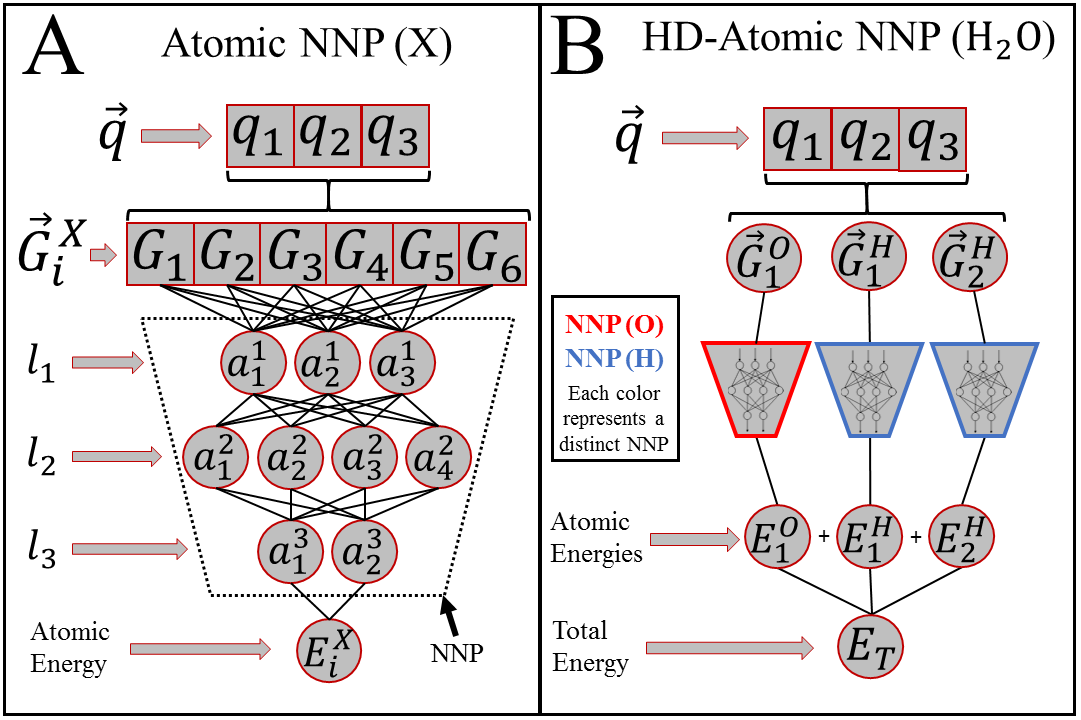
\includegraphics[width=\textwidth]{nn_ani}
      \par\hfill \tiny J. S. Smith, O. Isayev, A. E. Roitberg, ANI-1: An extensible nn potential with DFT accuracy
    \end{frame}

    \begin{frame}[c]\frametitle{Gvector Formula}
        
      \begin{align*}
        G^R_m &=\sum_{i\ne j}^{All Atoms} e^{-\eta (R_{ij}-R_S)^2} f_C(R_{ij})\\
        G^A_m &= 2^{1-\chi} \sum_{j,k \ne i}^{All Atoms} (1 + cos(\theta_{ijk} - \theta_S))^\chi  \\
        ~& \cdot exp\left[-\eta\left( \frac{R_{ij}+R_{ik}}{2}-R_S\right)^2\right] f_c(R_{ij})f_c(R_{ik})
      \end{align*}

      \begin{equation*}
        f_C(R_{ij})=
        \begin{cases}
           0.5 cos\left(\frac{\pi R_{ij}}{R_C}\right) + 0.5, & \mbox{for } R_{ij}\le R_C \\  
           0, & \mbox{for } R_{ij}\ge R_C \\  
        \end{cases}
      \end{equation*}
    
    \end{frame}

    \begin{frame}[c]\frametitle{Collecting the data}
        
      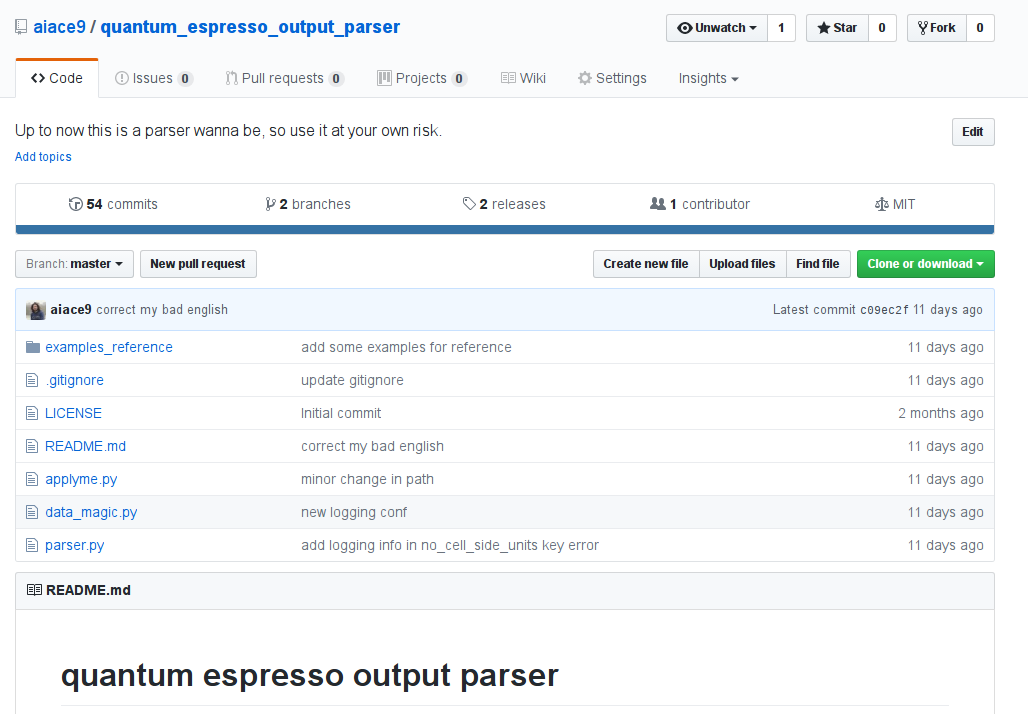
\includegraphics[width=\textwidth]{img/git_qe_parser.png}
    
    \end{frame}

    \begin{frame}[c]\frametitle{Implementation of the nn}

      \begin{columns}
        \column{.5\textwidth}
          
\includegraphics[width=\textwidth]{img/TF_logo.png}
        \column{.05\textwidth}
          %\begin{big}
            \textbf{+}
          %\end{big}
        \column{.28\textwidth}
          
\includegraphics[width=\textwidth]{img/py_logo.png}
      \end{columns}

      \par\hfill \tiny big thanks to Franco Pellegrini that wrote the Gvectors calculations an sketched the kernel of NN code

    \end{frame}
  % section what_we_are_developing (end)

  \section{where we are now} % (fold)
  \label{sec:where_we_are_now}

    \begin{frame}[c]\frametitle{Energy precision}
        
    Aim\footnotemark: $\left|E^{DFT}-E^{NN}\right|\sim$ \SI{2}{mRy/atom}\\
    Now: $\left|E^{DFT}-E^{NN}\right|= $\SI[separate-uncertainty = true]{10(10)}{mRy/atom}
    \footnotetext[1]{Result showed in the ANI paper}
    \end{frame}

    \begin{frame}[c]\frametitle{}
      
      \begin{center}
        Thank you for your attention
      \end{center}
    
    \end{frame}
  
    \begin{frame}[noframenumbering, c]\frametitle{What are we obtaining?}
    
      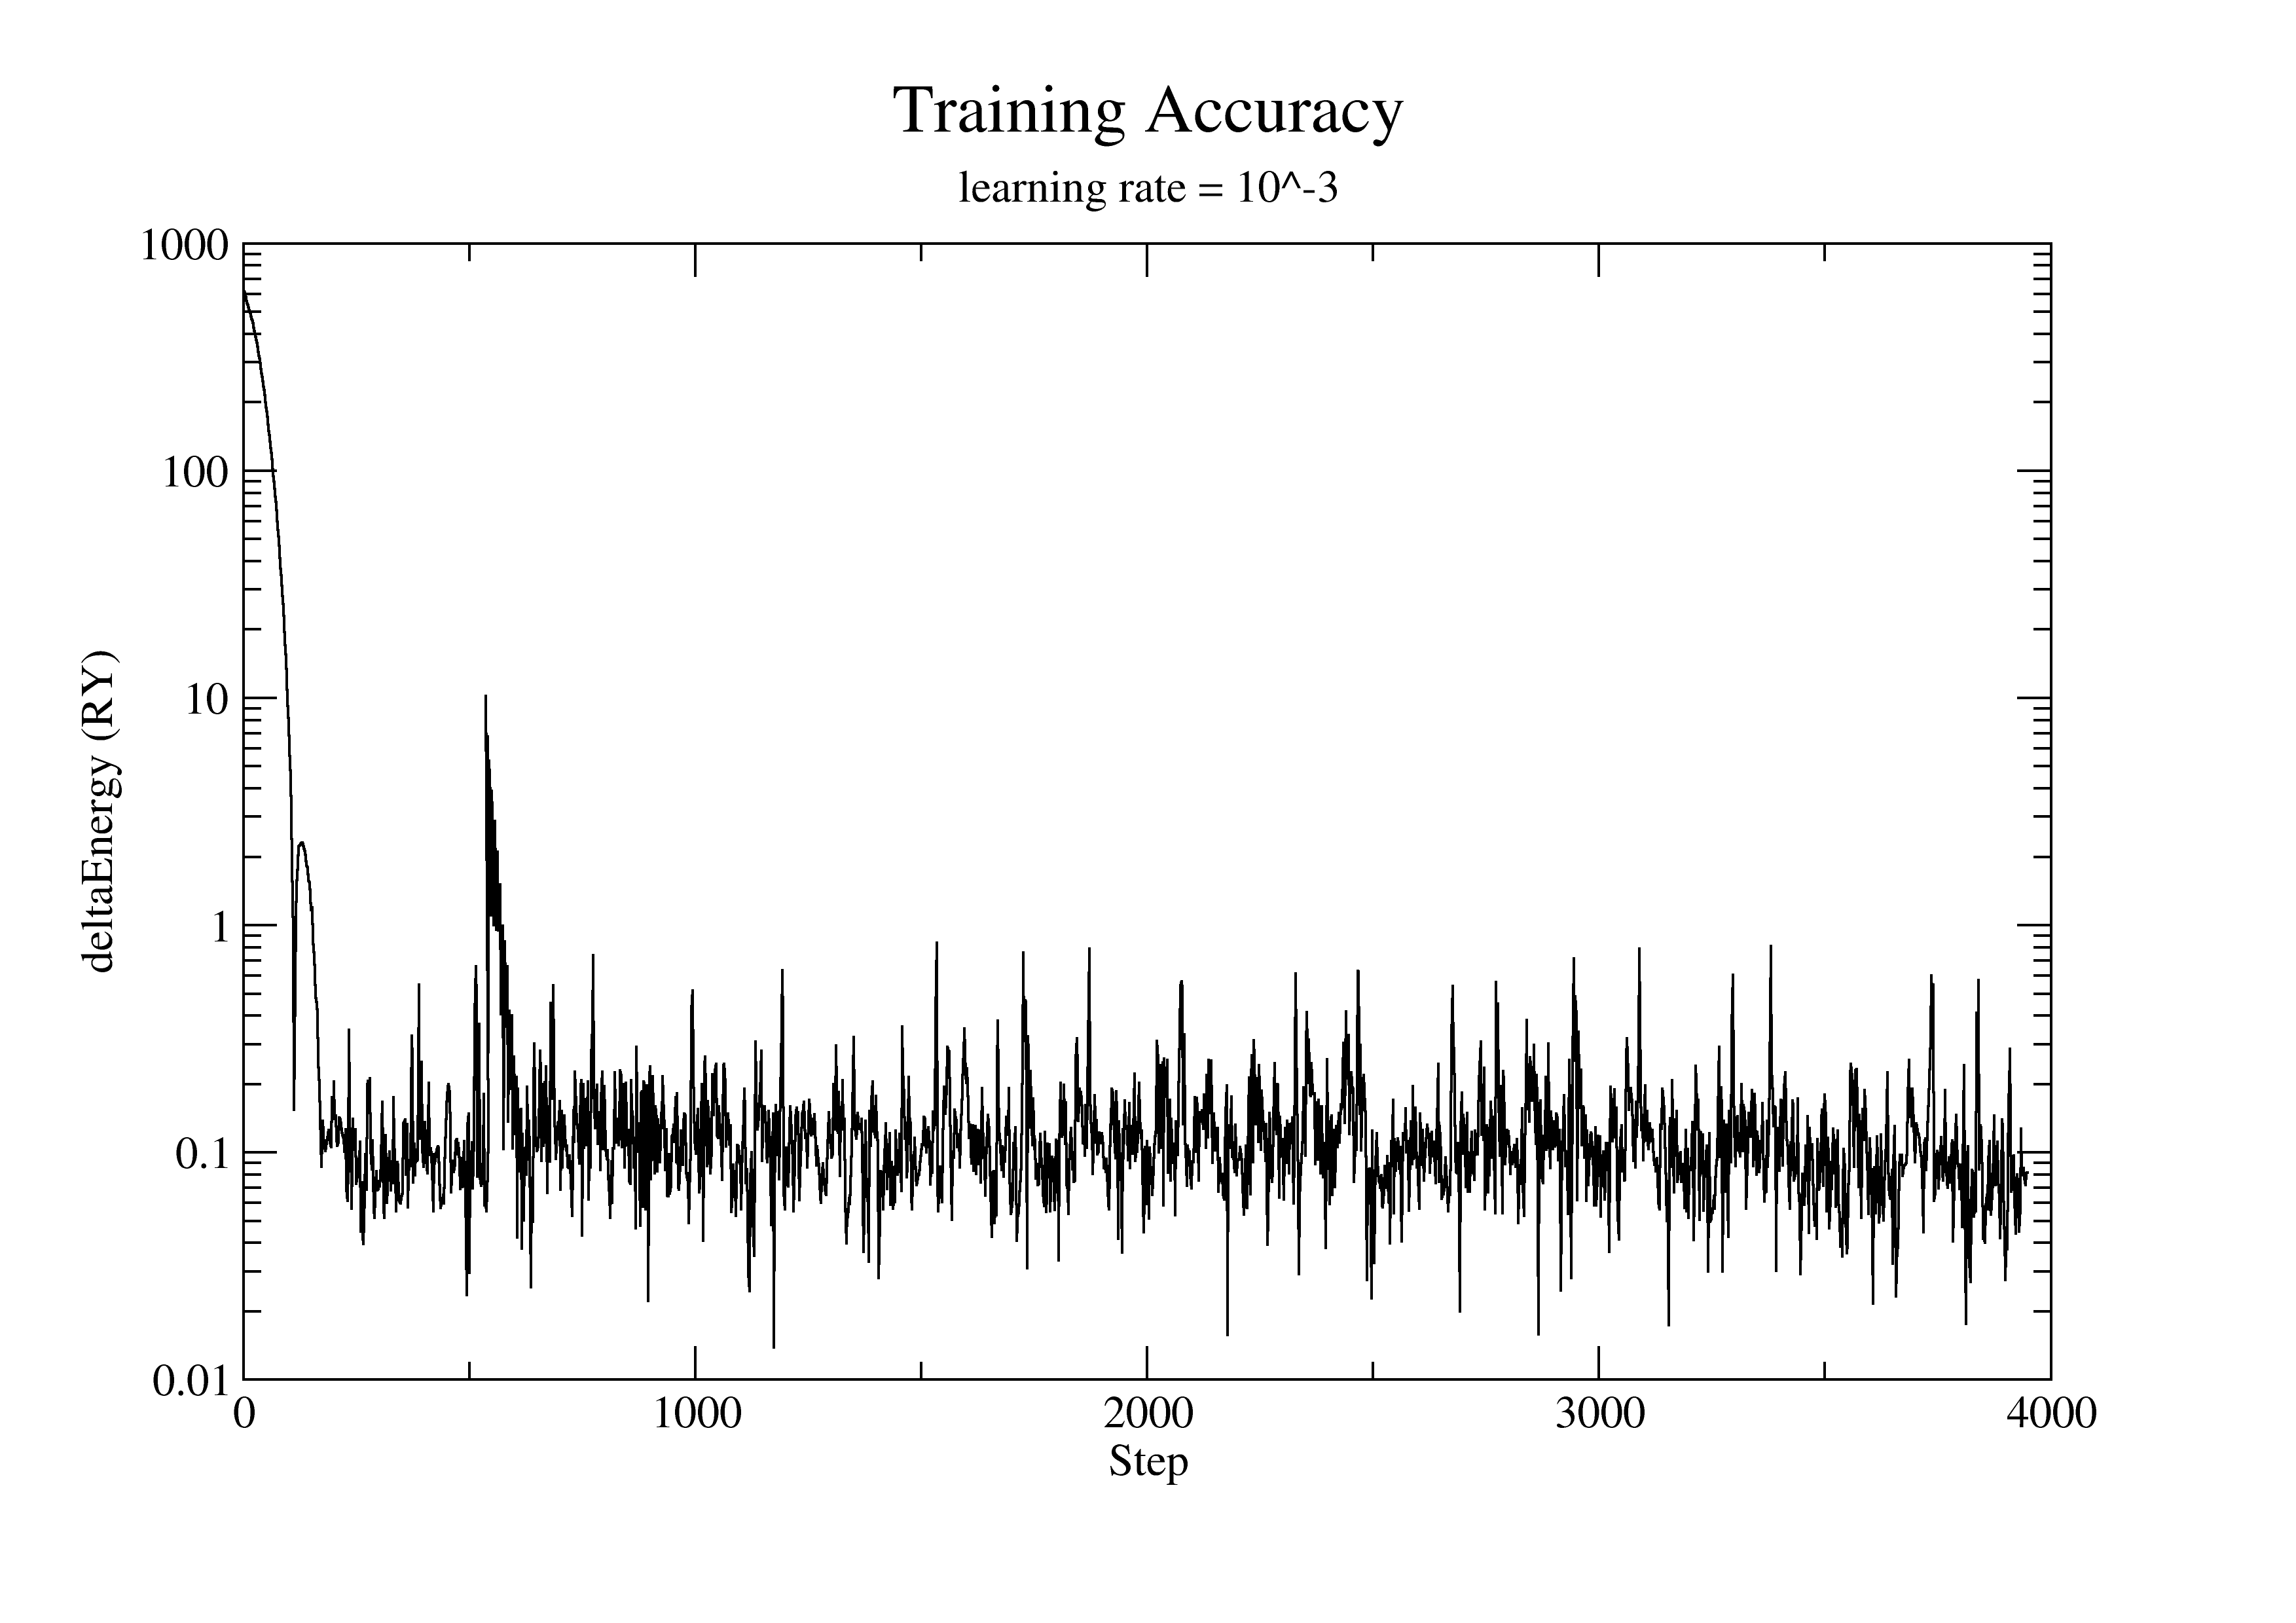
\includegraphics[width=\textwidth]{img/pres1.png}
    
    \end{frame}

    \begin{frame}[noframenumbering, c]\frametitle{What are we obtaining?}
    
      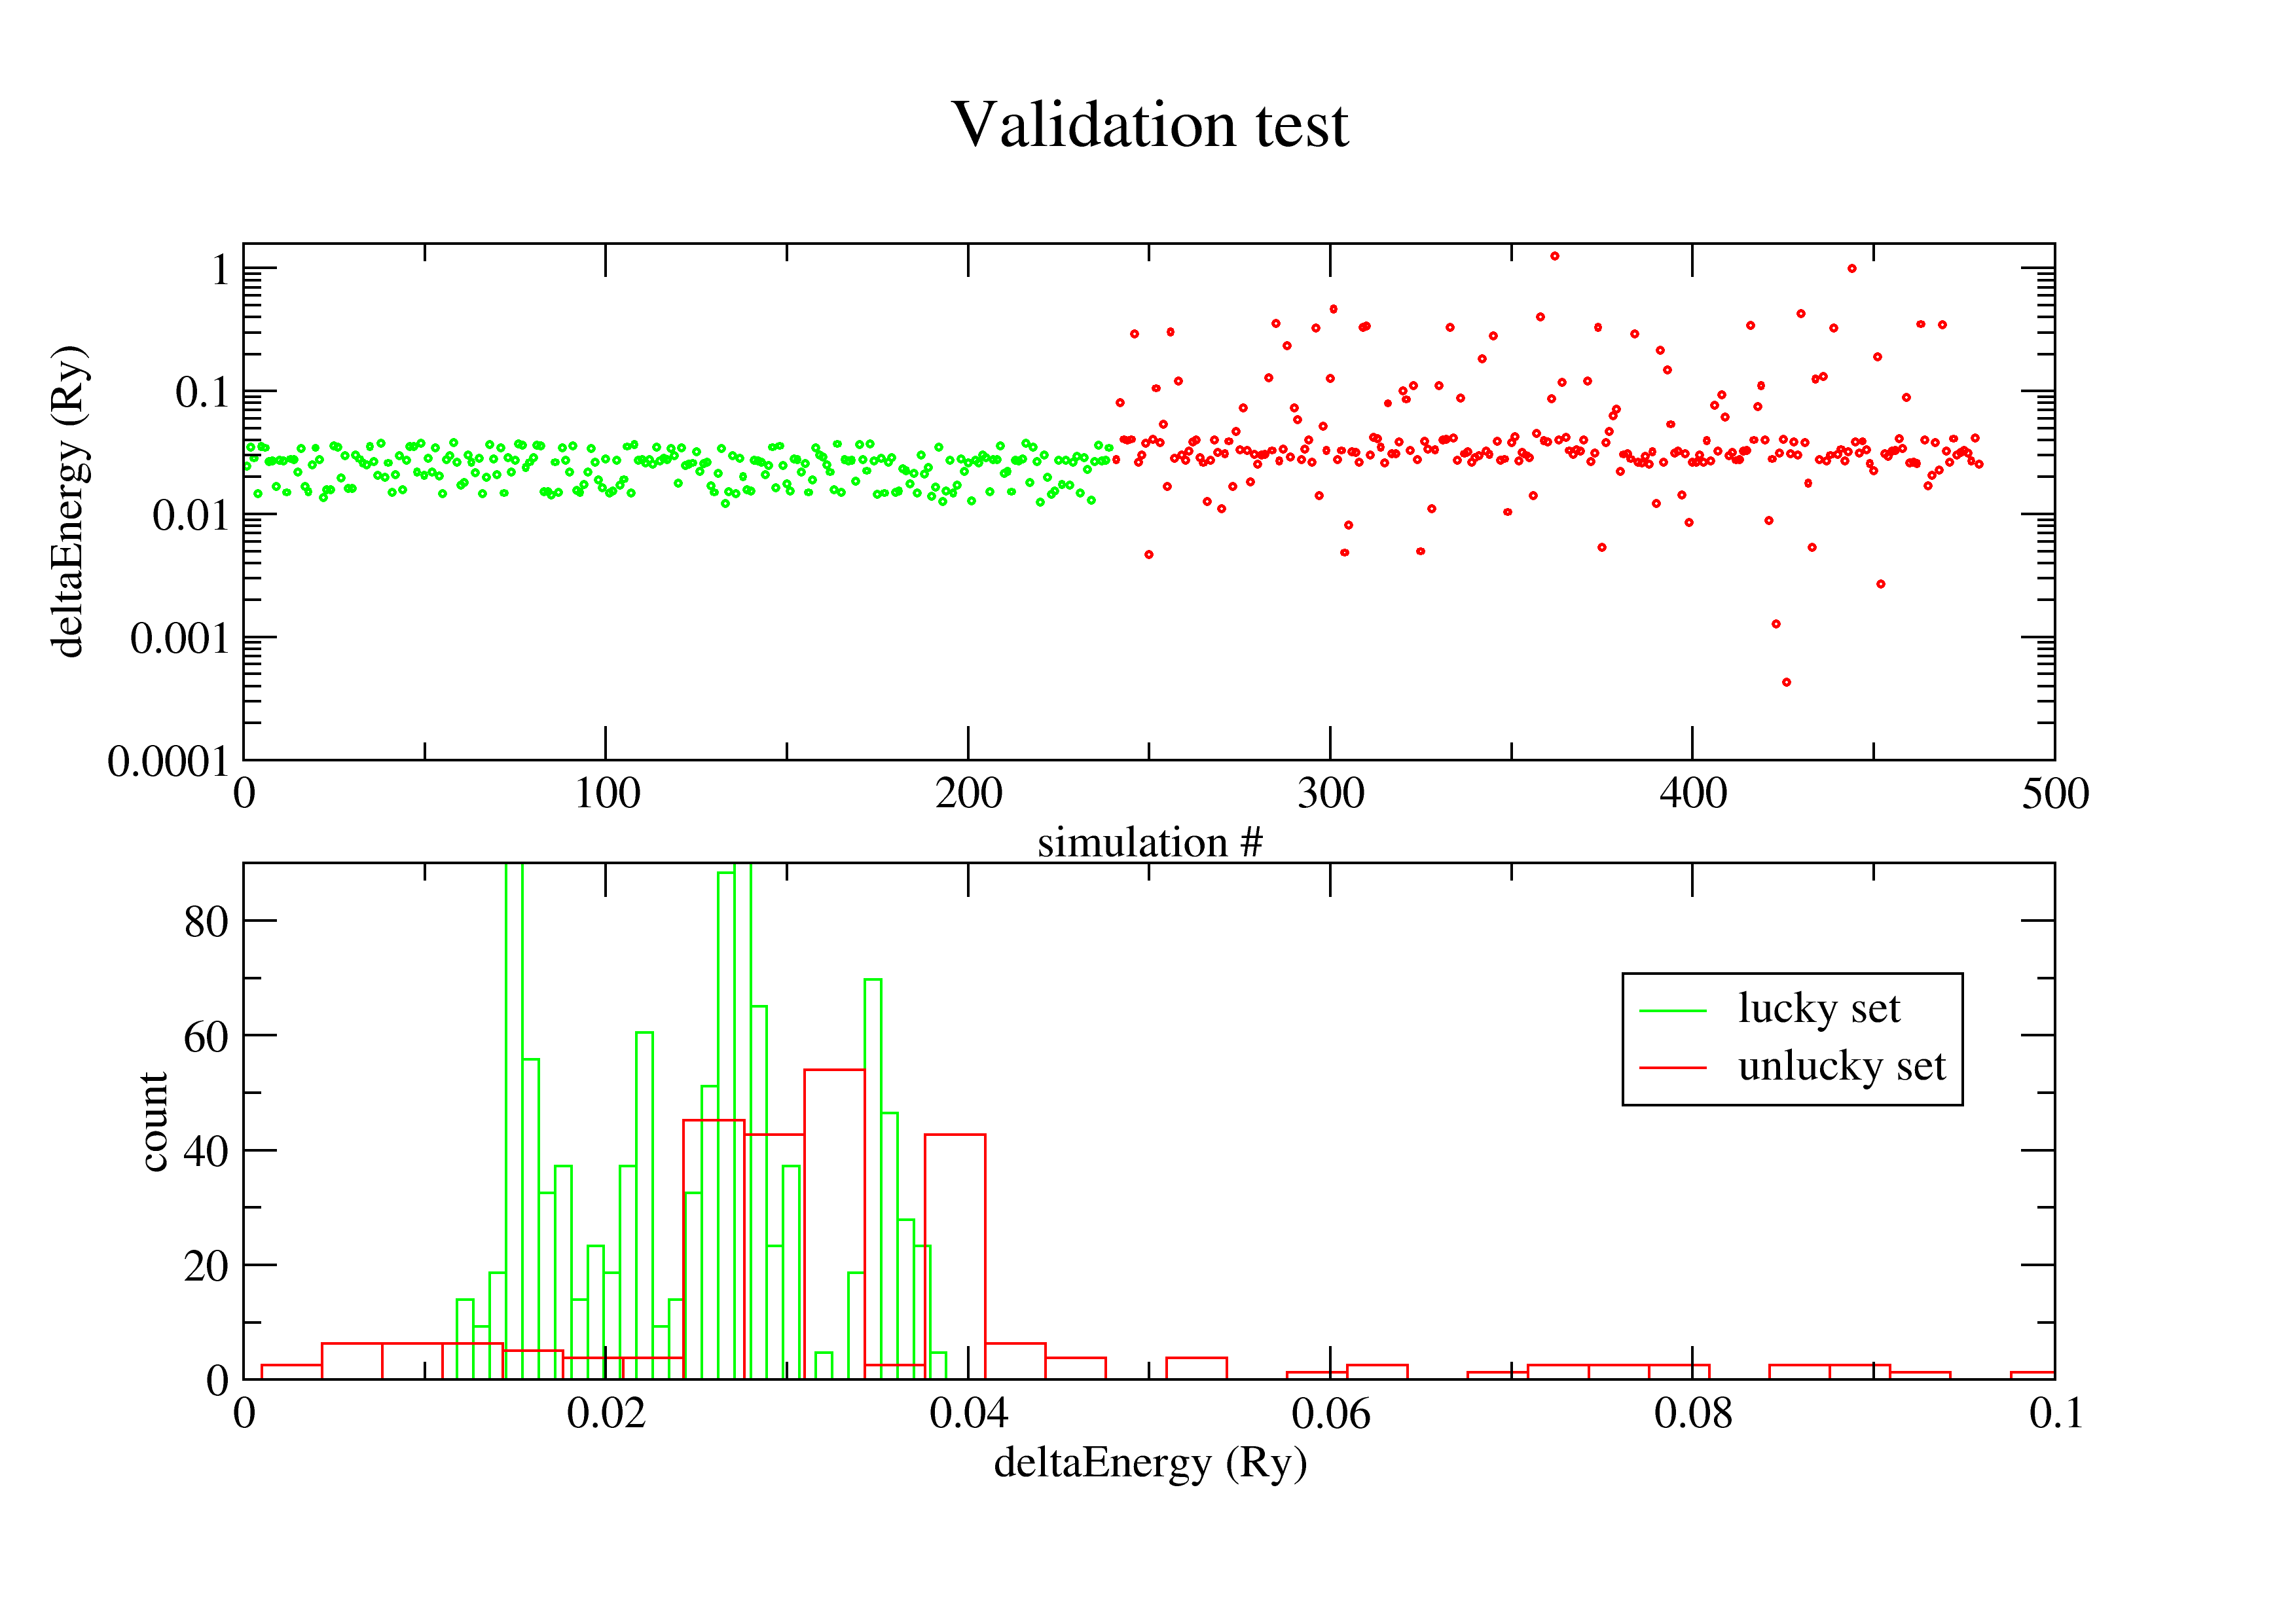
\includegraphics[width=\textwidth]{img/pres2.png}
    
    \end{frame}
  % section where_we_are_now (end)
\end{document}